%Edit 0020 ZZZ to report number nnnn 
%Edit  YYMILE to milestone number m.m.m
%Edit  Charter YYTITLE to report title - Words Start with Caps
\documentclass[11pt,twoside,a4paper]{article}
%%======================================================================
%% PACKAGES:
%%
%\usepackage{times}               % Times+Helvetica+Courier fonts
\usepackage{helvet}              % helvetica + cmr
%\usepackage{uarial}              % arial
\usepackage{fancyhdr}       % package for headers/footers
\usepackage{amsmath}
\usepackage{amssymb}
\usepackage{graphicx}            % Graphics.
%\usepackage{a4}                  % page layout to fit A4
%\usepackage{lastpage}            % get page no of last page
%\usepackage{ifthen}              % logical branching
\usepackage{hyperref}            %insert hyper-links
\usepackage{latexsym}
% uncomment the following to override auto page total
%\pptotal{20}
%%======================================================================

% ensure sans-serif font used throughout
\renewcommand{\familydefault}{\sfdefault}

\newcommand{\culhamissueno}{1.00}%<==edit
\newcommand{\culhamshorttitle}{CD/EXCALIBUR-FMS/0020}%<==edit
\newcommand{\Sec}[1]{Section~\ref{sec:#1}}
\newcommand{\Fig}[1]{Figure~\ref{fig:#1}}
\newcommand{\Tab}[1]{Table~\ref{tab:#1}}
\newcommand{\Eq}[1]{Equation~(\ref{eq:#1})}
\newcommand{\Eqs}[2]{Equations(\ref{eq:#1}) and~(\ref{eq:#2})}
\newcommand{\Figs}[2]{Figures~\ref{fig:#1}--~\ref{fig:#2}}
%Bold lc for script names, tt for computer code and file-names
%\F{NEPTUNE} always in caps
\newcommand{\F}[1]{\textsc{#1}}
\newcommand{\B}[1]{\textbf{#1}}
\newcommand{\T}[1]{{\tt #1}}
\newcommand{\V}[1]{\mathbf{#1}}
\newcommand{\I}[1]{\textit{#1}}
\newcommand{\nep}{\textsc{NEPTUNE}}
\newcommand{\exc}{\textsc{E}x\textsc{CALIBUR}}
\newcommand{\Papp}{Proxyapp}
\newcommand{\papp}{proxyapp}



%%======================================================================

%% REPORT COVER PAGE Information

\newcommand{\culhamtitle}{\LARGE \exc \ \nep \ Charter }%<==edit

%%QA BOX information -- change following as needed
\newcommand{\culhamboardname}{Martin O'Brien}%<==edit
\newcommand{\culhamcontactname}{Rob Akers}%<==edit
\newcommand{\culhamauthor}{Wayne Arter}%<==edit
\newcommand{\culhamauthora}{Ed Threlfall}%<==edit
\newcommand{\culhamauthorb}{Joseph Parker}%<==edit
\newcommand{\culhamauthorc}{Debasmita Samaddar}%<==edit
%\newcommand{\culhamcontacttel}{Telephone: 01235 466498}
%\newcommand{\culhamcontactemail}{Email: rob.akers@ukaea.uk}

\newcommand{\culhamdate}{7 September 2020}%<=edit
\newcommand{\culhamdatea}{7 September 2020}%<=edit
\newcommand{\culhamdateb}{7 September 2020}%<=edit

% reproduce Rob's page size

\setlength{\textheight}{220.0mm}
\setlength{\textwidth}{165.0mm}
\setlength{\topmargin}{0.0mm}
\setlength{\oddsidemargin}{0.0mm}
\setlength{\evensidemargin}{\oddsidemargin}
\setlength{\parindent}{0mm}
\addtolength{\parskip}{0.5\baselineskip}
\setlength{\topsep}{0pt}
\setlength{\itemsep}{0pt}

%%======================================================================
\begin{document}

%Titlepage comes out wrong size, but should look right apart from
% picture which cannot be wider than c.150mm.
% To produce conforming report rp1pub.pdf
% remove title page by commenting out lines ending in %<==omit, then
% sed -e '/<==omit$/s/^/%/' < rp1.tex > rp1omit.tex
% pdflatex rp1omit;bibtex rp1omit; pdflatex rp1omit
% pdfunite cover.pdf rp1omit.pdf rp1pub.pdf 
\begin{titlepage}%<==omit
\vspace*{-30mm}%<==omit

\includegraphics[width=2.5cm]{../corpics/cofaplus} \\[2.0\baselineskip]%<==omit
{\LARGE {\textbf{\textsf{ExCALIBUR}}}}\\[2.0\baselineskip]%<==omit
{\LARGE \culhamtitle } \\[2.0\baselineskip]%<==omit
{\textbf{\textsf{Abstract}}}\\%<==omit
This is the charter for \exc \ project \nep.%<==omit
The report describes equations for \exc \ project \nep \ \Papp s.  
The numbering of the systems follows that of the \nep\ Science Plan, so 
that those listed under FM-WP2 are denoted 2-1, 2-2, etc., and 
under FM-WP3 as 3-1, 3-2, etc. It is a living document to which further equation 
systems will be added throughout the course of the project.
%<==omit
%<==omit
\vfill%<==omit
\centerline{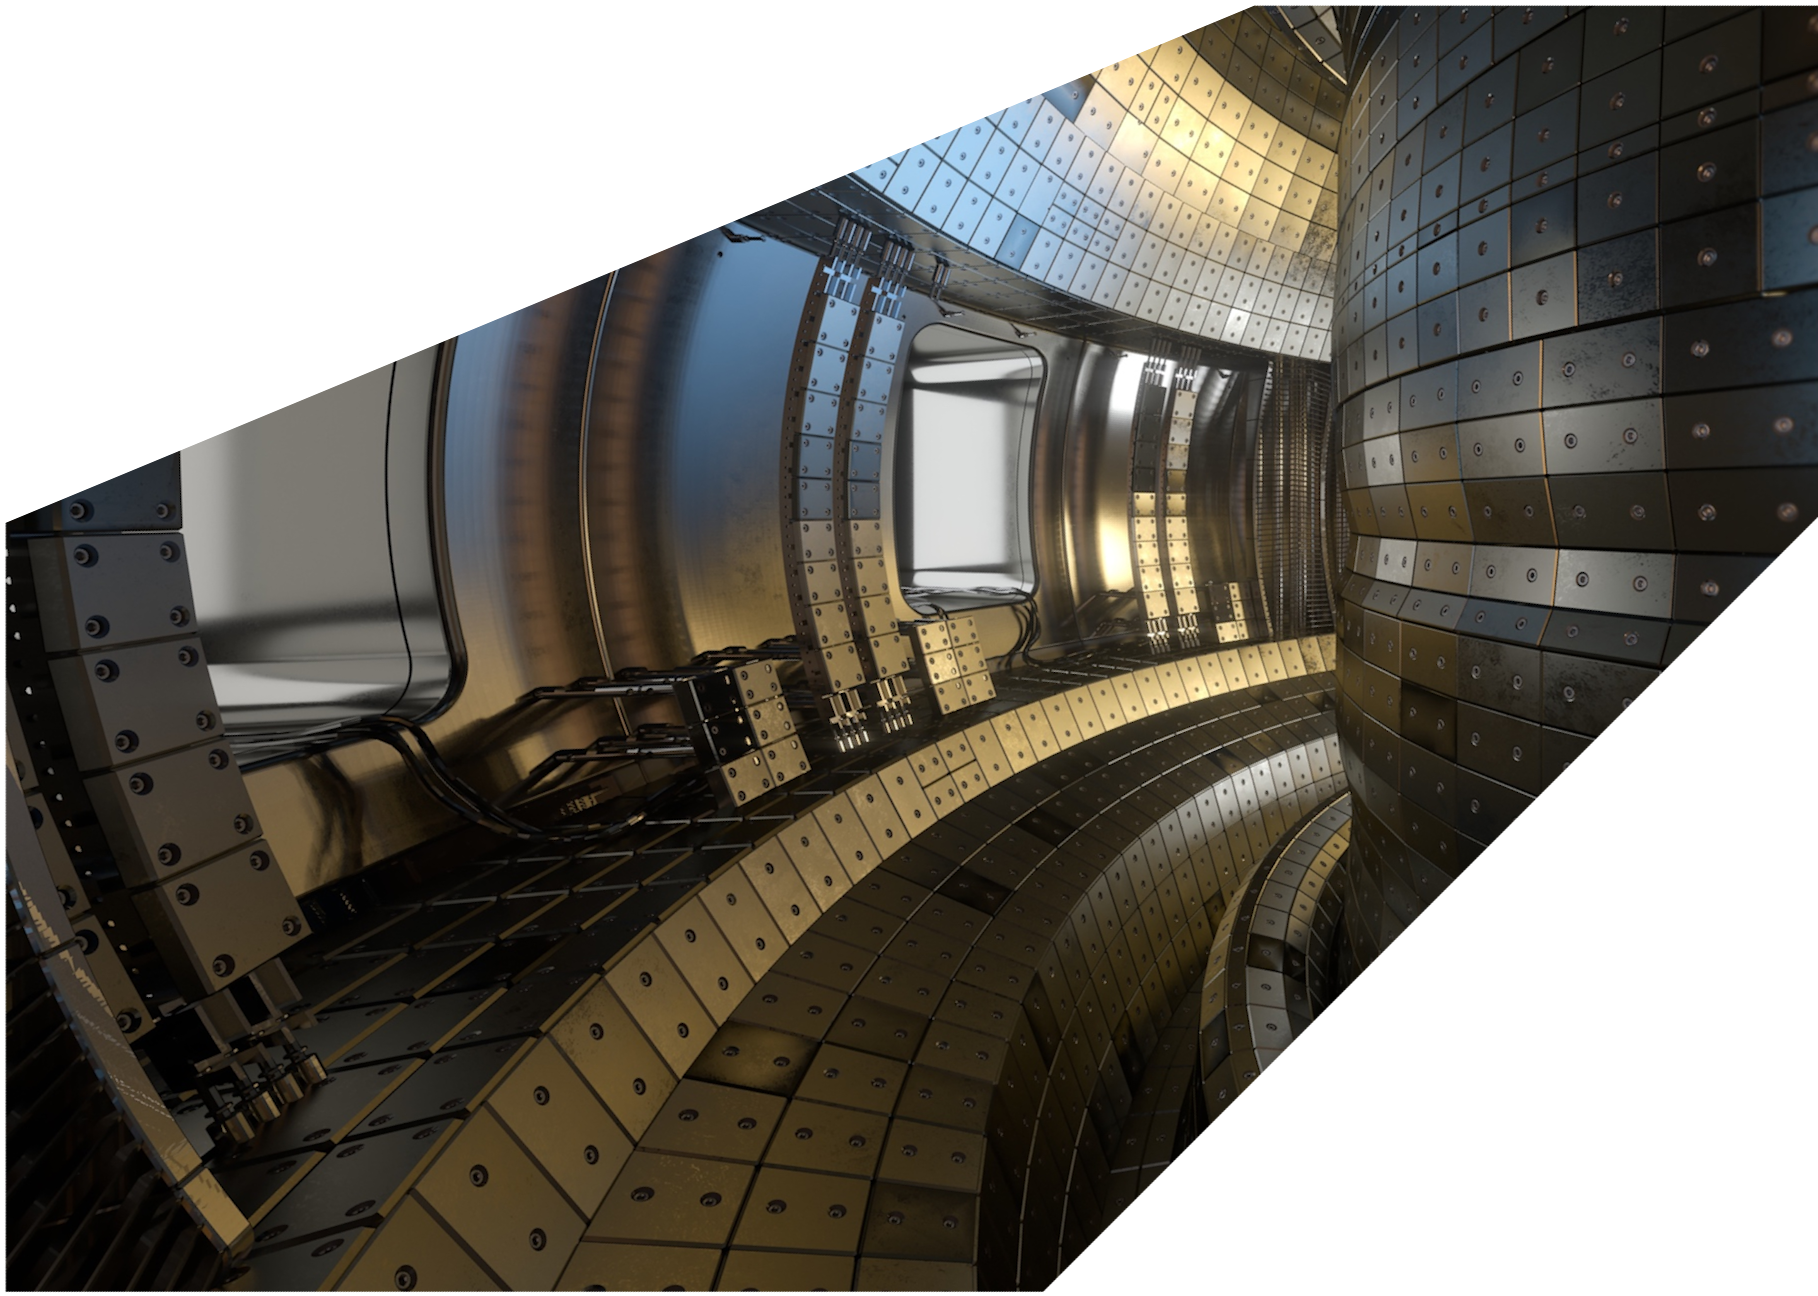
\includegraphics[width=0.9\textwidth]{../corpics/tokintcrop}}%<==omit
\end{titlepage}%<==omit

\hspace{-30mm}\begin{table}[h]
\sffamily
\begin{center}
\textbf{\textsf{UKAEA REFERENCE AND APPROVAL SHEET}}
\begin{tabular}{||p{5.7cm}|p{4.7cm}|p{5.0cm}||}
\hline
\hline
& Client Reference: &  \\
\hline
& UKAEA Reference: & \culhamshorttitle \\
& & \\
\hline
& Issue: & \culhamissueno \\
\hline
& Date: & \culhamdateb \\
\hline
\multicolumn{3}{||l||}{} \\
\multicolumn{3}{||l||}{Project Name: ExCALIBUR Fusion Modelling System} \\
\multicolumn{3}{||l||}{} \\
\hline
\end{tabular}
\begin{tabular}{||p{3.3cm}|p{4.6cm}|p{3.5cm}|p{3.6cm}||}
\hline
& Name and Department & Signature & Date \\
\hline
Prepared By: & \culhamauthora & N/A & \culhamdate \\
& \culhamauthor & N/A & \culhamdate \\
%& \culhamauthorb  & N/A & \culhamdate \\
%& \culhamauthorc  & N/A & \culhamdate \\
& & & \\
& BD & & \\
\hline
Reviewed By: & \culhamcontactname & 
\includegraphics[width=3.0cm]{../corpics/blanksign}& \culhamdatea \\
& & & \\
& Advanced Computing Dept. Manager & & \\
\hline
%Approved By: & \culhamboardname  & \includegraphics[width=3.0cm]{../corpics/mobsign} & \culhamdateb \\
%& & & \\
%& MSSC & &\\
%\hline
\hline
\end{tabular}
\end{center}
\end{table}
%<==omit

%\clearpage
%\section{Introduction}\label{sec:intro}
%The edge region is in parts a very good vacuum, so 
that the plasma ion species typically do not thermalise fully.
Nonetheless it may be adequate for many purposes to treat the majority ionised species as fluids,
although this is harder to argue for impurity species that may be present only in relatively
small numbers.
In fact, collision timescales typically vary $\tau\propto T^{3/2}/N$ where $T$ is the temperature of the species
and~$N$ is its number density, so that a species may be treatable as a fluid over say microsecond
timescales in cooler, denser regions, but not on shorter timescales or in parts closer to the core.
There is the additional complication of sheath formation at the edge, where the preferential
loss of electrons leads to strong electric fields and consequently flows close to sonic,
so that most workers model the sheath plasma using particles, typically with the Particle-in-Cell~(PIC)
approach, although for the Vlasov equation a wide range of numerical techniques has been examined,
see eg.\ Palmroth~et~al~\cite[\S\,4]{Pa18Vlas}.
\emph{N.B. Discussion in this note implies usage of particles to model kinetic effects,
not schemes such as SPH designed to model advection of classical fluids.}

The cooler parts of the tokamak edge plasma may contain large numbers of
neutral atoms.
Neutrals are generically less likely than charged species to thermalise.
They circulate into hotter and denser regions and collide with charged species.
Classical transport coefficients~$\kappa$, in
addition to a~$1/\tau$ dependence, are anisotropic because of the strong magnetic field,
to the extent that collisions with neutrals may become an important limiting mechanism
for transport along the field. Operationally the most important aspect of the
neutral species is however that because of the collisions, they
represent a source of plasma.

The non-Maxwellian or kinetic aspects of the edge may lead to a need to solve the
Boltzmann equation, in fact not only with quadratic source terms representing interaction
between two species colliding, but with cubic terms representing chemical reactions.
Classical fluid dynamics of course assumes Maxwellian dependence on phase velocity and
concentrates on the first few moments  density, mean flow and sometimes temperature
as well as pressure. It can be helpful to introduce
the concept of phase-fluid, where extra dimensions represent the velocity-space
dependence at a position in full detail.
In the phase-fluid approach, the concept of multiplicatively perturbing
a Maxwellian has been explored. The main and important advantage of this approach
is that it often facilitates massive simplification of the collision integrals
in Boltzmann, to a single point term in significant cases, eg.\ ref~\cite{zhdanov}.

Kormann, with Yurova and others (private communication, 2019) have recently reviewed the use of 
the Hermite basis (ie.\ a Gaussian multiplied by a Hermite polynomial). Two
significant works are Vencels et al.~\cite{Ve16Spec} describing Spectralplasmasolver
and J.T.Parker's thesis~\cite{jtparker} which describes software focused on
gyroaveraged kinetics, namely SPECTROGK. Note that all these works use a Fourier
representation for real space, the so-called Fourier-Hermite method.
%, so that additional development would be needed for \nep

Even with the simplification of a multiply-periodic domain,
there are nonetheless issues particularly at high velocity values
and of course a Maxwellian may not be a particularly good approximation. 
Hence, borrowing from classical CFD practice on a infinite domain, it might be
interesting to look at mappings which expand a set of compact spectral elements to cover
the whole of velocity space.

\begin{figure}
\centerline{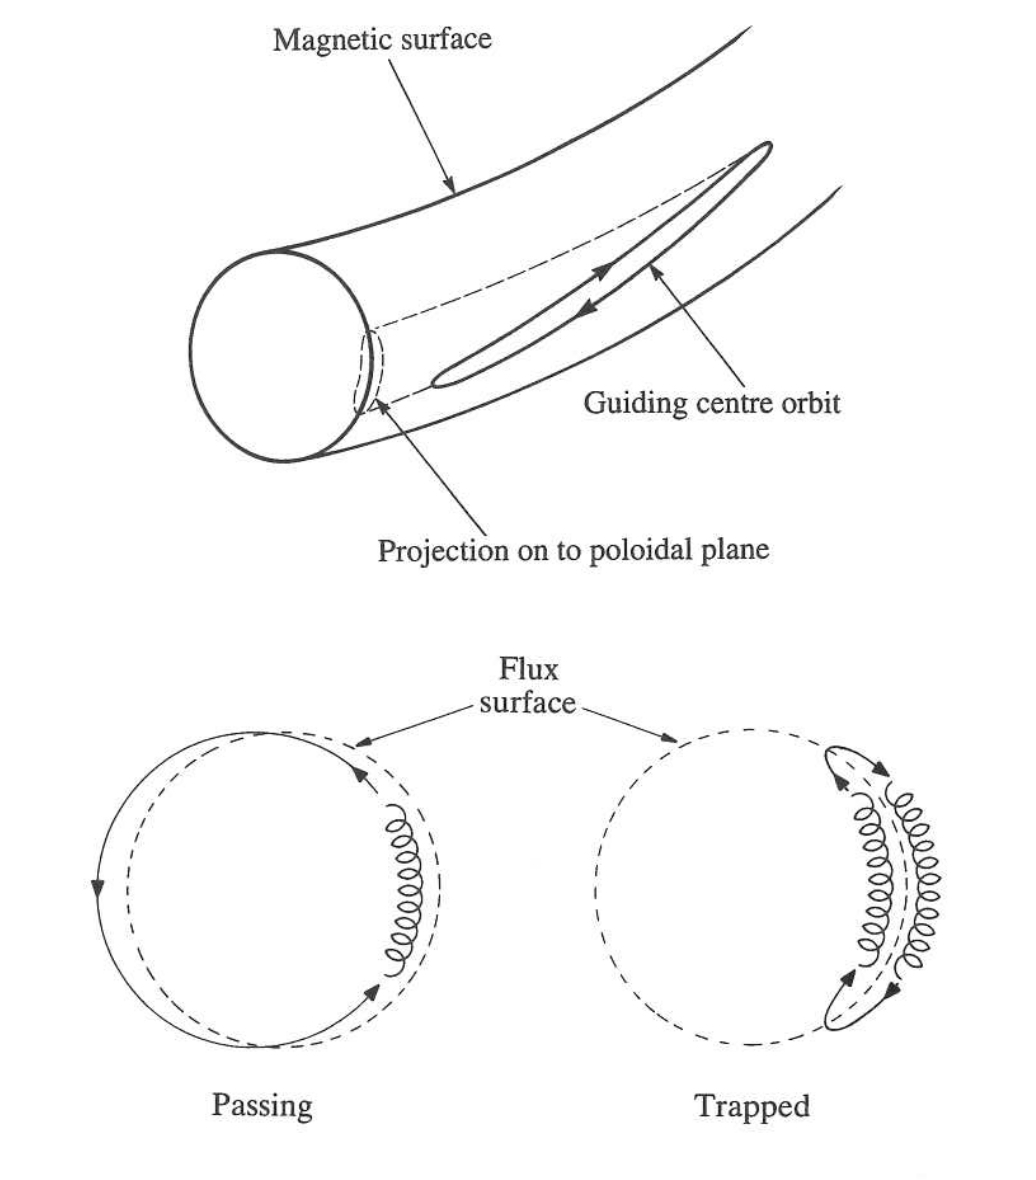
\includegraphics[width=8cm]{../png/pcle_orbits}}
\caption{Important classes of particle trajectories from Wesson~\cite[\S\,3.10]{wesson}.\label{fig:orbits}}
\end{figure}

Alternatively it may be easier to return to basics and look at a particle representation
for the ionised species as well as for the neutrals. This
may be as efficient as using higher order elements since the distribution function in velocity may not be
very smooth. As the sketch in \Fig{orbits} indicates, there are two important classes of particle
trajectories, depending on the particle energy and where in the magnetic field they begin.
The first set approximately follow the fieldlines, gyrating as they go, whereas the second set
may have trajectories that bounce. There is lack of smoothness at the trapped-passing
boundary in velocity space.


%The need to use particle as well as fluid models, puts a significant burden on the software,
%because it gives rise to a general need to be able to move between representations without
%introducing excessive error.

%\clearpage
\section*{\exc \ \nep \ Charter}\label{sec:taskwork}
There are two basic approaches to meshing a B-rep,
namely (1) to represent the geometry by means of `voxels'\cite{Bu07Trea},
or (2) to mesh the surface, then generate a volume mesh that coincides with
the surface mesh.

\begin{figure}
\centerline{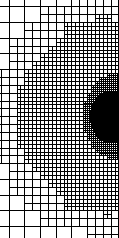
\includegraphics[width=8cm]{../png/amrmesh}}
\caption{An AMR mesh surrounding a curved body drawn as solid black at right.\label{fig:amr}}
\end{figure}
Voxels are the volume equivalent of pixels, so that the geometry
is represented by a uniform cuboid lattice of geometrically
identical cells, each possibly labelled with a set of physical properties.
Refinements of voxelisation are to allow
clusters of small cells to be treated as larger
cuboid bodies~\cite{Va05CTan}, and to omit cells altogether within say solid surfaces
(also known as `tartan meshing'). When both techniques are combined in say CFD,
the result is known as an AMR mesh, see \Fig{amr}.

\begin{figure}
\centerline{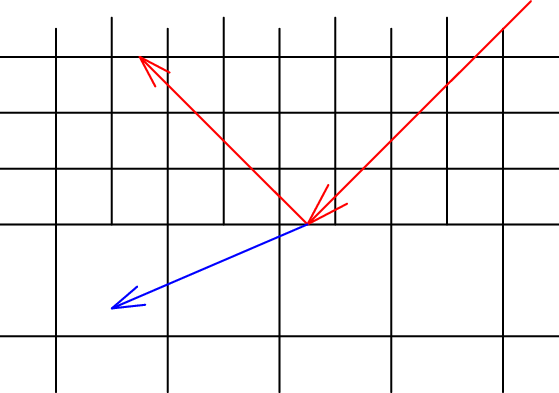
\includegraphics[width=8cm]{../png/iamr}}
\caption{Spurious reflections when using low order scheme with AMR\label{fig:amrefl}}
\end{figure}

As suggested by the previous paragraph, an AMR mesher is potentially quite complicated.
A well-known difficulty with schemes that use AMR meshes is illustrated by \Fig{amrefl}.
There will be interfaces between meshes of different size, even in regions with
the same physical properties. However, a wave with a wavelength of less than~$10h$, where
$h$ is the local mesh-spacing, modelled using a second-order accurate scheme,
has a propagation speed in error by~$1$\,\%, which
error increases as $h^p$~typically with $p=2$. Thus computationally, the
region show in \Fig{amrefl} may have different dispersion properties at
shorter wavelength in the two different grid-sizes, and computations will
exhibit a spurious reflection at the interface, which may be misleading or even
destabilising in certain cases.
The importance of the work of Nikiforakis et al~\cite{Go18Dime} is that they
have managed to produce in effect a spatio-temporal AMR mesh, so that they can
compute the equations of inviscid compressible FD \emph{explicitly} using a local timestep.
Such meshes have also been successfully used for Particle-in-Cell calculations of
extreme complexity for spacecraft charging~\cite{Mi16part}, meaning that Nikiforakis
work deserved attention. Unfortunately,
considerable discussion of the merits of the Nikiforakis approach versus spectral
element at the Birmingham meeting~\cite{y1re111b} indicated potentially severe difficulties for
AMR meshes when diffusion, especially anisotropic diffusion has to be treated.

\subsection{Importance of Geometrical Accuracy} \label{sec:codegeom}
The approximate nature of the intersection between two NURBS surfaces may also cause
difficulties, as indicated by \Fig{meshes}. Power deposition
on the PFCs shielding may depend critically on the direction of the surface normal.
A grid of planar triangles may produce errors like those indicated by
\Fig{meshes}(a), whereas more faithful representations would resemble
\Fig{meshes}(b).
\begin{figure}[h]
\centerline{(a){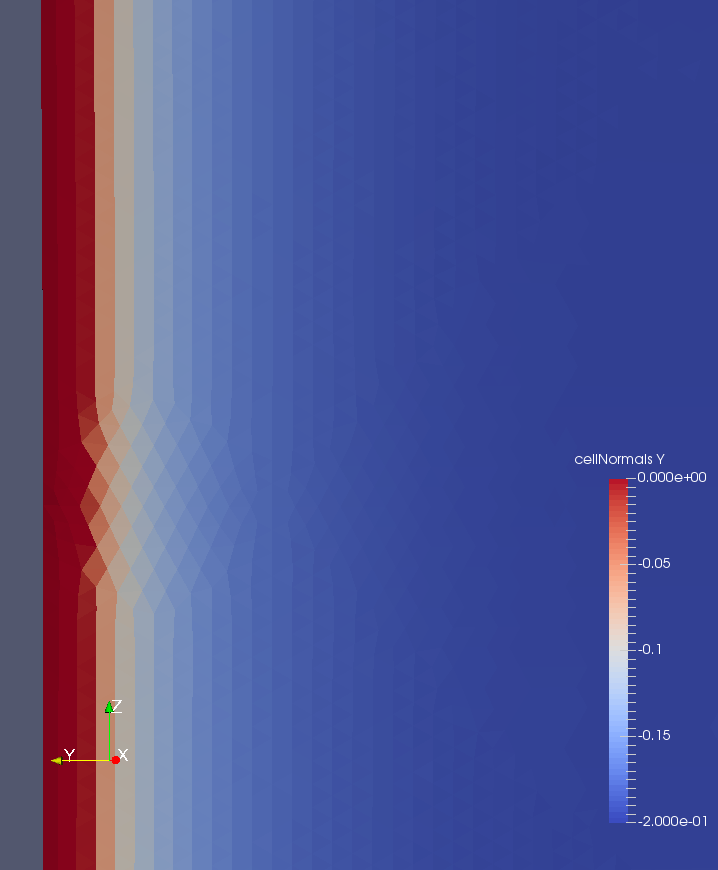
\includegraphics[width=7.0cm]{../png/meshbad.png}}
(b) {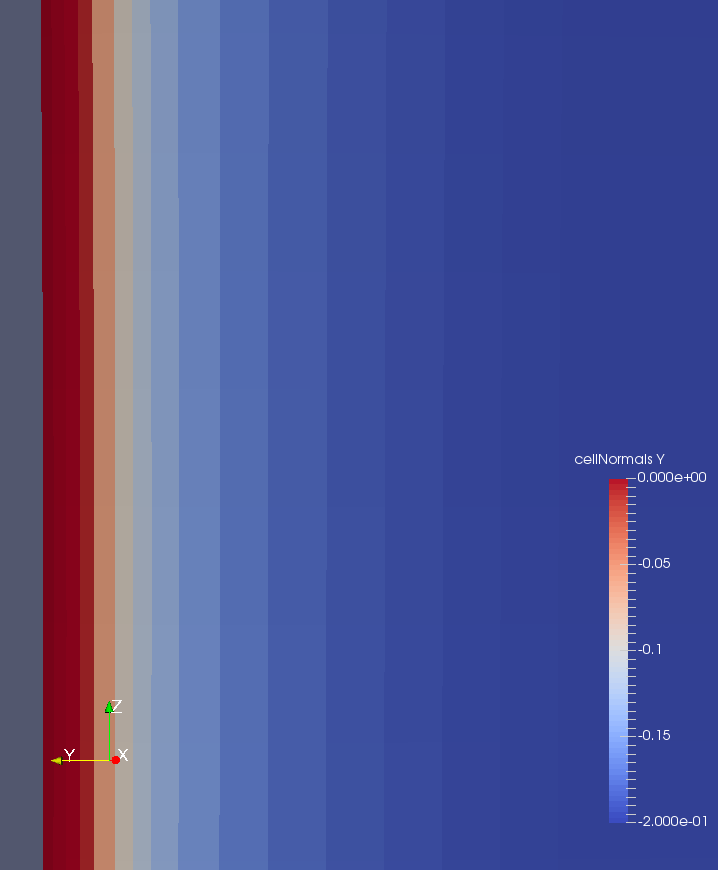
\includegraphics[width=7.0cm]{../png/meshgood.png}}
}
\caption{Close-ups of two triangular meshes of the central left edge surface
of a TBM Tungsten shield.  The  CAD contains a join in the middle of the image
leading to the irregular behaviour of the horizontal component of surface normal
in the image at left~(a). Refitting of CAD using the CADfix$^{TM}$ software package
enables the production of a more smoothly
varying normal, see mesh at right~(b).
\label{fig:meshes}}
\end{figure}



A difficulty for both AMR and surface-based approaches is the order of error~$p_s$ in the spatial approximation of
surfaces and other interfaces used to bound the domain of a PDE calculation.
The important result is by Boffi~\cite{Bo12Infl} that
the results of a PDE calculation can have order no higher than~$p_s$. Thus in the
usual approach that starts by meshing the surface with simple planar triangles, there is
no point in using schemes of high or spectral order. Many  meshing packages allow only for
second order surface approximations, whereby typically each side of say a `curved' triangle is 
represented by three points and hence a quadratic fit. Notable exceptions
are gmsh~\cite{Ge09gmsh} and MFEM~\cite{Do20hrad,mfemwebsite}.

\begin{figure}
\centerline{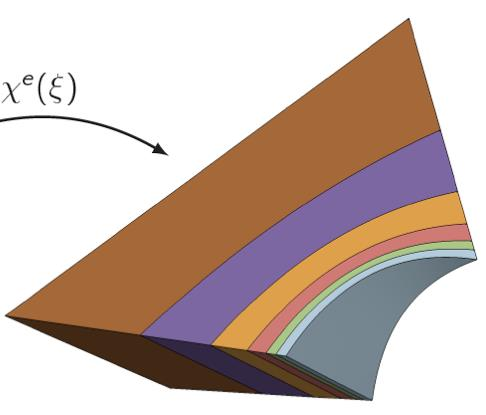
\includegraphics[width=8cm]{../png/shmo-754}}
\centerline{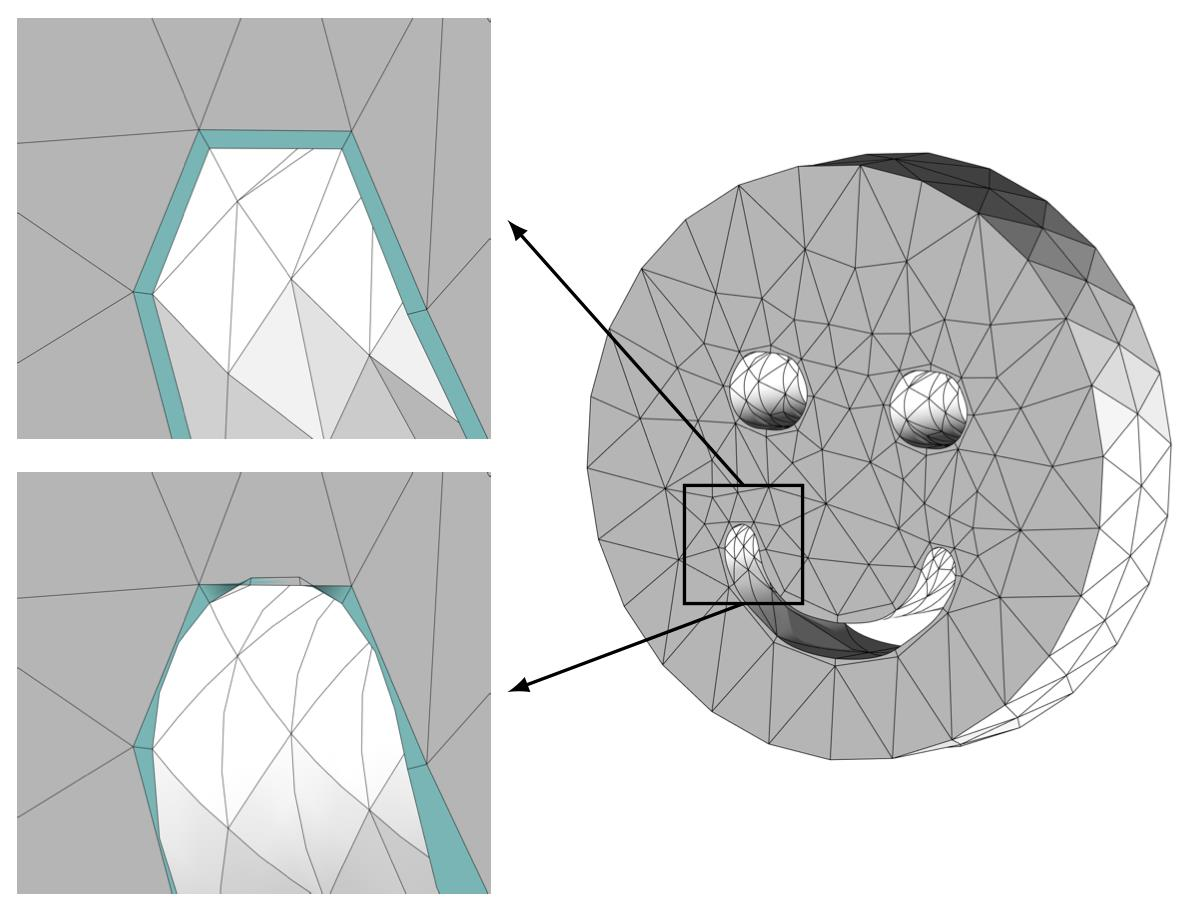
\includegraphics[width=8cm]{../png/shmo-672}}
\centerline{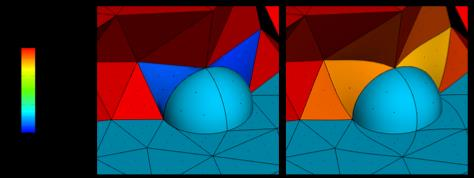
\includegraphics[width=8cm]{../png/shmo-681}}
\caption{At top is illustrated a desirable meshing close to a curved surface, when eg.\ small
scale physical effects due to a sheath need to be represented. Below is an indication
of how packages may fail when they try to produce this mesh using low-order spatially
spatially accurate elements (planar triangles), from a presentation by Sherwin and Moxey
at CCFE\label{fig:meshprob}
At bottom is a second picture from the same presentation, showing resolution
of a problem arising when mesh is tangent to a surface.}
\end{figure}

Consultations indicate difficulties with higher-order spatially accurate meshing
even for relatively simple geometries that might be encountered in the tokamak edge.
\Fig{meshprob} shows two problems. The first is where  self-intersection occurs when
trying to insert nodes  inside thin elements near curved boundaries. The other is
where the surface triangulation has a tangency to an extrusion. The Nekmesh
software is being developed~\cite{Tu17fram,Tu18Curv} using concepts from optimisation theory to 
treat such issues.

\clearpage
\subsection{Example Meshing Problem} \label{sec:meshprob}
A example text case is formed by the meshing of the surface JET Tile~1~(T1),
which is one of the vertical tiles at the left of the divertor in \Fig{jetdive}.
The figures containing surface meshes are taken from a study in ref~[RP4,\S\,5.1]\cite{Wa19}
that attempted to find a minimal, accurate mesh representation for the 
T1 surfaces receiving power.
\begin{figure}
\centerline{
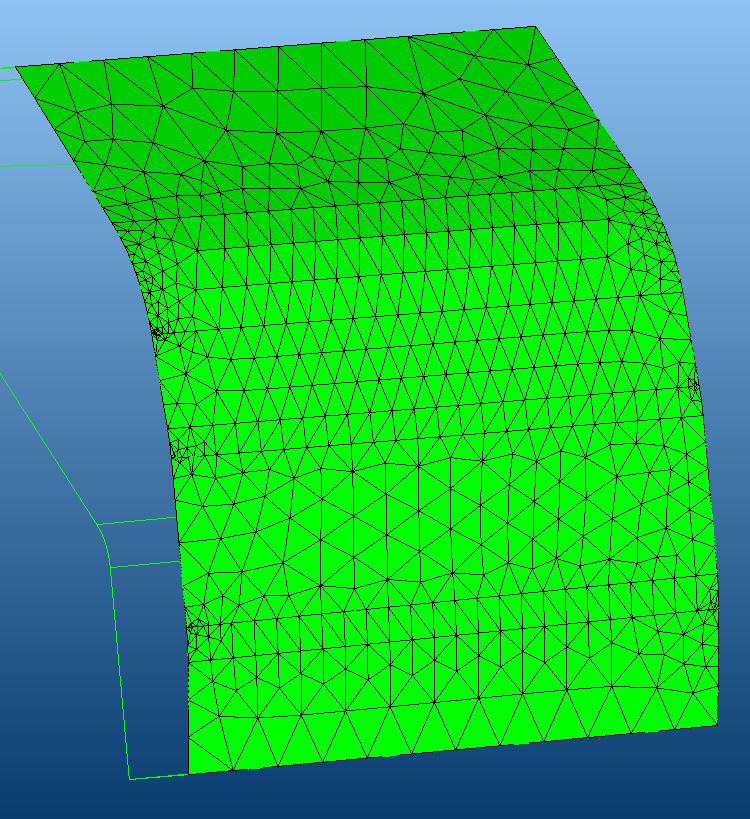
\includegraphics[width=0.42\columnwidth]{../png/t2t5}
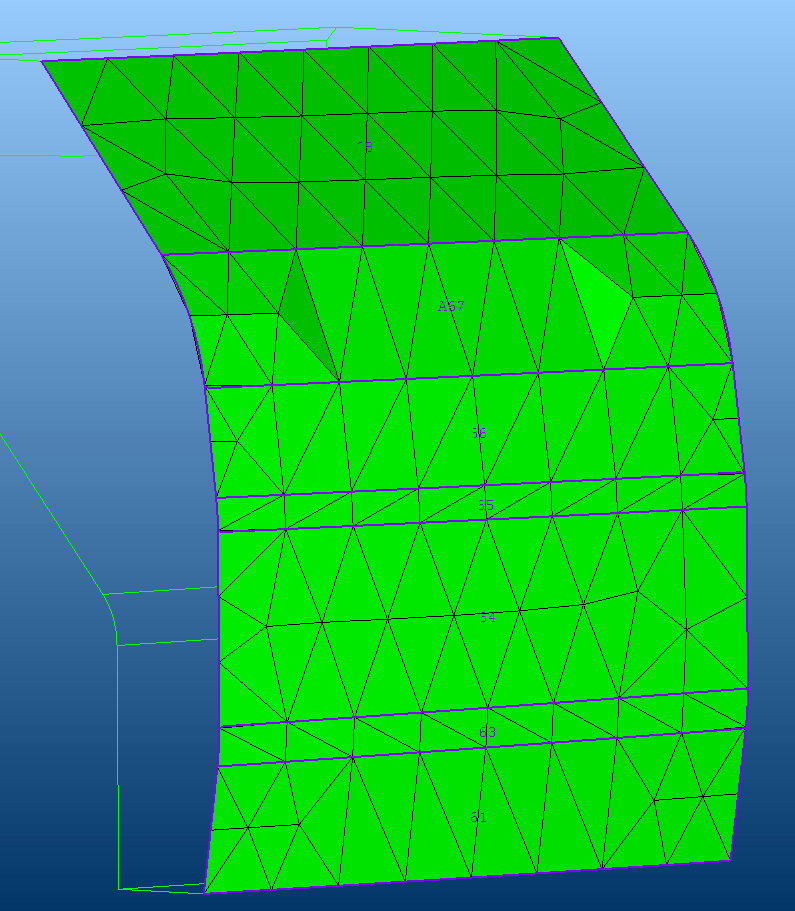
\includegraphics[width=0.4\columnwidth]{../png/t2t2}
}
\caption{
Different T1 meshes produced with (left) and without sag control (right).
The left plot has mesh features illustrates the gap between boundaing NURBS curve and NURBS surface,
caused in this case by defeaturing of fillets around the surface edges.
\label{fig:meshsag}}
\end{figure}

%32

\begin{figure}
\centerline{
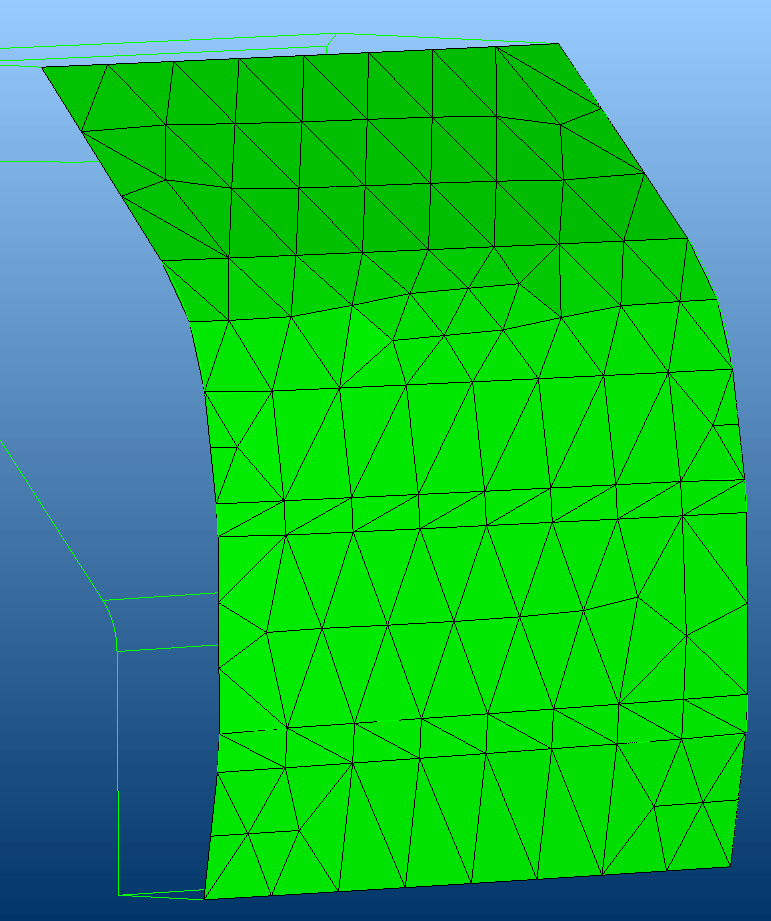
\includegraphics[width=0.33\columnwidth]{../png/t2t1}
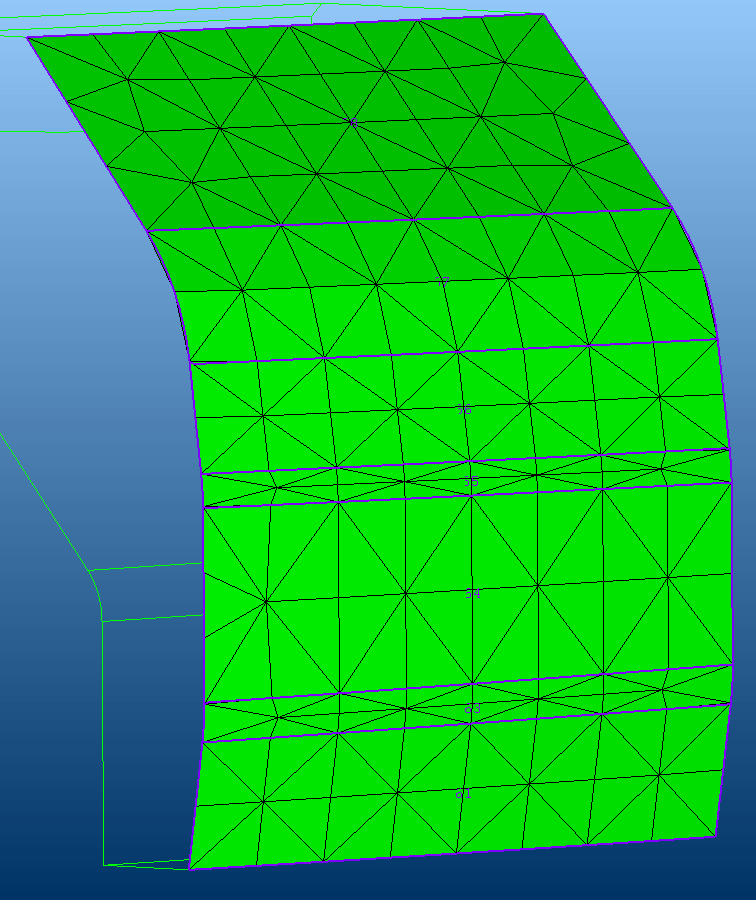
\includegraphics[width=0.33\columnwidth]{../png/t2t3}
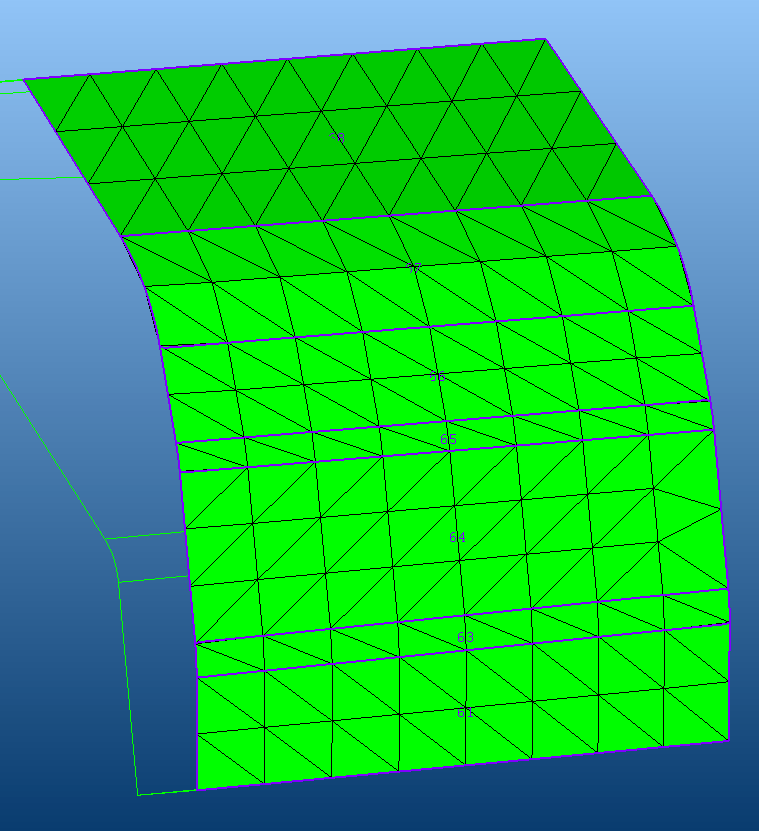
\includegraphics[width=0.35\columnwidth]{../png/t2t4}
}
\caption{
Exploration of the effect of different meshing controls on T1.
\label{fig:meshopt}}
\end{figure}

\begin{figure}
\centerline{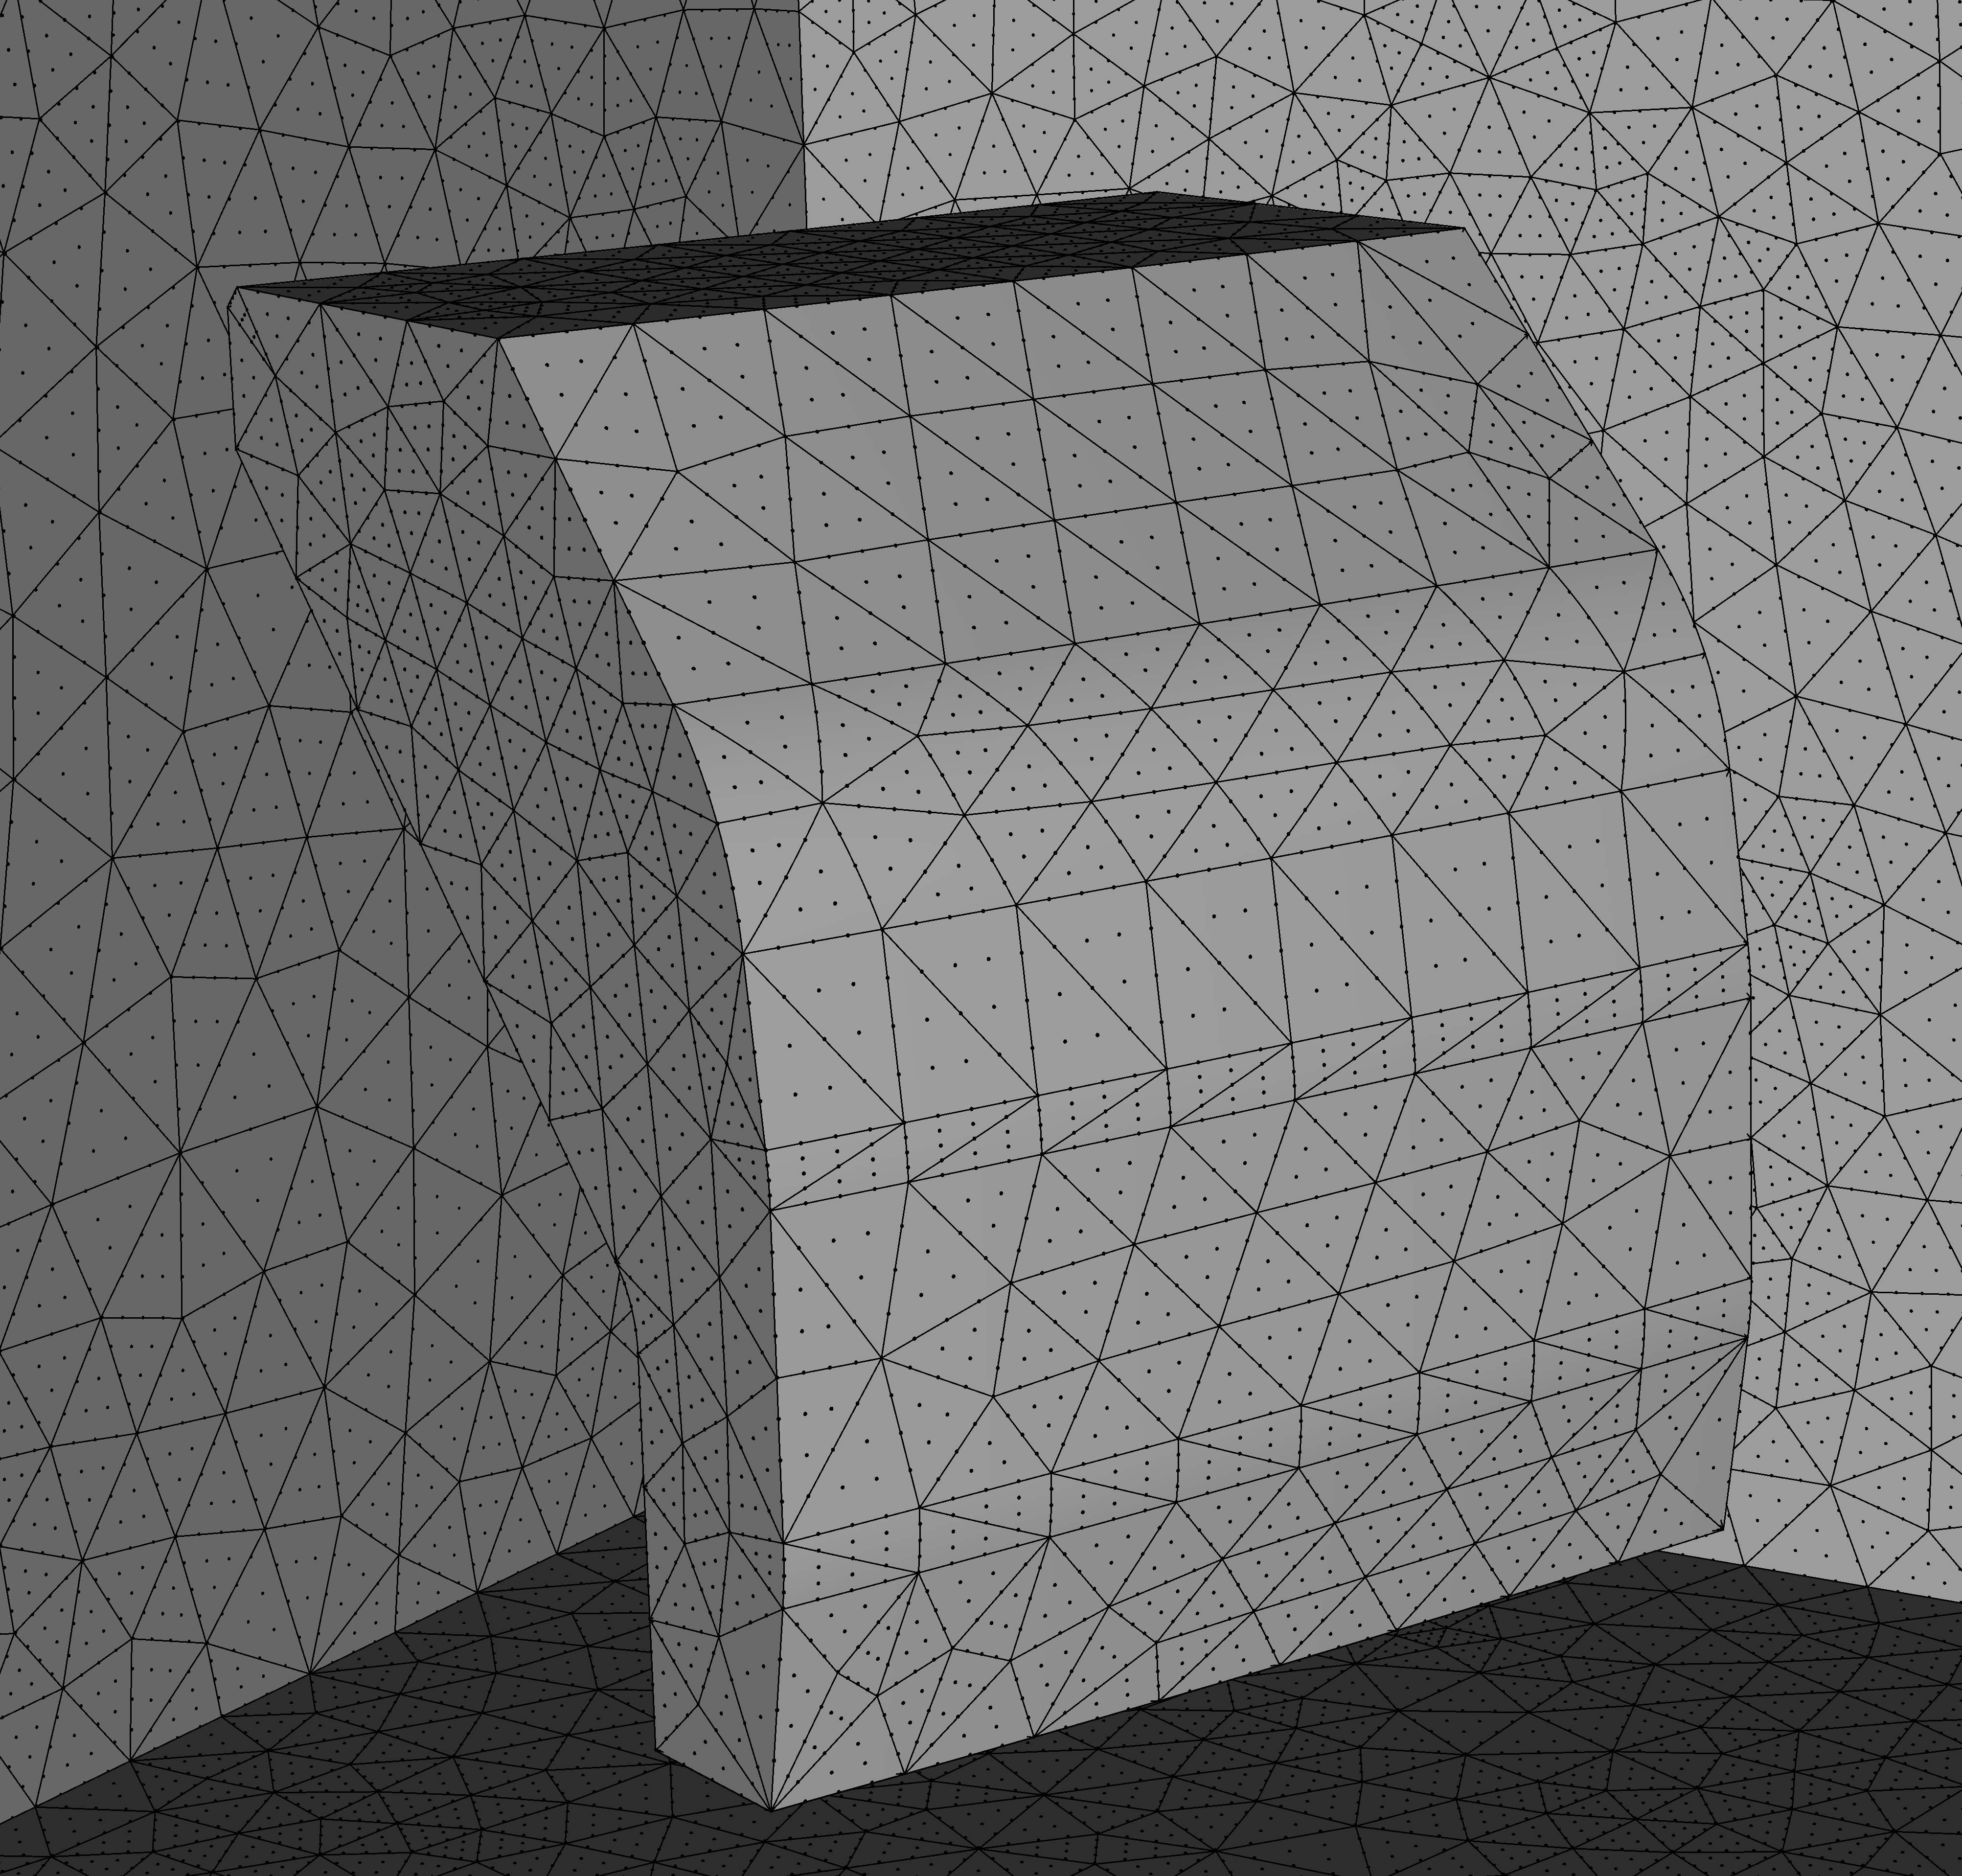
\includegraphics[width=8cm]{../png/visit0000}}
\caption{Meshing of JET T1 tile by D.~Moxey 6/3/20 using Nekmesh. The dots indicate nodes within
the non-planar triangular elements.\label{fig:visit0}}
\end{figure}


A sample text case is illustrated in \Fig{visit0} for the JET Tile~1,
which is one of the vertical tiles at the left of the divertor in \Fig{jetdive}.

\clearpage
\subsection{Element Shape Problem} \label{sec:eltprob}
\begin{figure}
\centerline{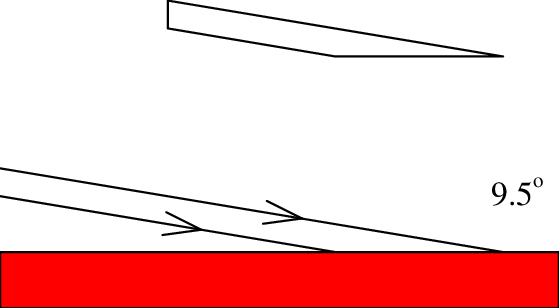
\includegraphics[width=8cm]{../png/9p5deg}}
\caption{Undesirable element shape if meshing conforms to both surface and fieldline.\label{fig:9p5deg}}
\end{figure}

Even assuming accurate meshing, there is a problem caused by the need to spread power
as widely as possible over the surfaces. Power is observed to flow along field lines, being
deposited proportionately as $\hat{\bf n}\cdot(\hat{\bf B}$, where  $\hat{\bf n}$ is
the unit normal to the surface and $(\hat{\bf B}$ gives
the direction of magnetic field~${\bf B}$.
Many designs call for a $2^o$~angle of field incidence on the surface. Such a small angle
is impossible to draw, the best that
is easily drawn is $9.5^o$ ($\arctan 1/6$), see \Fig{9p5deg} Elements with $2^o$ corners present such serious
challenges that simultaneous alignment with both the fieldlines and the geometry appears
to be a non-starter. The Science Plan~\cite{sciplan} recognises that it will be important to establish just
how large an anisotropy in the transport can be treated accurately without special coding.

%Fluid model of the edge : challenges
%1. Flow into engineered tile surface at
%approx. sonic speed following field
%Two-degree incidence design cf. 9.5o
%2. Magnetic field causes anisotropy
%3. Interaction with neutrals leads to large sources and sinks of mass and momentum
%4. Neutral particles are not necessarily Maxwellian distributed
%5. Plasma ion species often not accurately represented as fluid either
%6. Fluids may be 5-D or 6-D phase-fluids as well as 1-D to 3-D


\clearpage
\begin{table}[h]
\textbf{\textsf{GLOSSARY:}}
\begin{center}
\begin{tabular}{|p{4.0cm}|p{12.0cm}|}
\hline
\textbf{\textsf{Term or Acronym}}
& \textbf{\textsf{Definition}} \\
C++ & Programming language, see \url{https://isocpp.org/} \\
DPC++ & Data Parallel C++, Intel compiler for C++ with SYCL extension \\
DSL & Domain Specific Language, programming language developed for a specific area of resrearch and development \\
Object Fortran & Programming language, more precisely Fortran~95 or later exploiting object-oriented features of the language, see \url{https://wg5-fortran.org/f2008.html} \\
Python & Programming language, see \url{https://python.org/} \\
SYCL & C++ library  for portable high performance computing, see \url{https://www.khronos.org/sycl/} \\
Kokkos & C++ library for portable high performance computing \url{https://cfwebprod.sandia.gov/cfdocs/CompResearch/docs/Kokkos-Multi-CoE.pdf} \\
OpenMP & Software for parallel programming \\
SRO & Senior Responsible Owner role in UK  government project delivery \\
Julia & Programming language, see \url{https://julialang.org/} \\
UKRI & United Kingdom Research and Innovation, a non-departmental public body encompassing the research councils and Innovate UK \\
VVUQ & Verification, Validation and Uncertainty Quantification \\
\hline
\end{tabular}
\end{center}
\end{table}

%\section{Summary}\label{sec:summ}
%The requirements capture exercise did not raise any significant issues that
had not been anticipated in the Science Plan~\cite{sciplan}.
Concerning modelling and software, there was remarkably little dissension.
The question of the physics to be included has been settled in the
short term  by the need to align with the E-TASC projects on edge modelling.
Longer term there are questions still to be resolved concerning the
details of the gyroaveraged kinetic (or other kinetic) model to be employed,
the inclusion of special relativistic effects, plasma chemistry, 
and for example whether the PFC boundaries should be allowed to `melt',
and whether particle dynamics within the top layers of PFCs should be included.

There is still a debate about how best to deal with situations when the software
even at the Exascale is incapable of resolving boundary or internal layers.
A feature of the lower order (Patankar) fd scheme is that it can be
formulated so that in an implicit time advance of a field advection-diffusion equation,
it acts a contraction mapping on the field, ie.\ it converges to a single, finite solution,
regardless of lack of layer resolution or of size of timestep. Under such circumstances, a spectral
scheme may fail completely cf.\ the dispersion analyses of say Ainsworth et al~\cite{Ai09Disp}
and more recently for spectral/hp element schemes in the Galerkin~\cite{Mo16Eige} and 
discontinuous Galerkin~\cite{Mo15line} contexts,
and users generally prefer an answer to none at all.
Of course, it may be argued that a manifestly erroneous result without an accuracy estimate
will not be used to action large procurements, but in any event it would be better
for the spectral scheme to produce a result at increasingly extreme parameters.

There are a number of ways to achieve this, the most obvious' being the use of
explicit artifical viscosity,
to broaden thinner layers or small features to the
point where full spectral accuracy is achievable.
Different options have been explored, of
which the most robust appears to be `DG-mimicking spectral vanishing viscosity'~ (SVV), see ref~\cite{Mo19Spat}.
Fernandez et al~\cite{Fe19Nonm} specifically addresses robustness when mesh resolution becomes poor..

A better approach from the point-of-view
of accuracy is to insert more resolution (more elements or increased order polynomials)
where aliasing error has been detected. This has its limitations in terms of cost,
but there are also practical issues concerning refinement that still need investigation.
Some of these latter points might be more easily addressed by reformulating the problem 
in terms of a variational approach and/or using the Lie derivative formulation~\cite{La03prac}.
It was anticipated that these could be addressed in the cross-cutting programme.

Interaction with a reactor design framework awaits better definition of data structures
for such tools. There seems no reason however why this should not be addressed inside-out,
as regardless, techniques have to be produced for moving data at the Exascale.

Subject to the above qualifications, the production of proxyapps should proceed in Y2 as indicated
in the Activities Plan~\cite{y12acts}, viz.\ a larger task :
\begin{itemize}
\item to define a referent physics model for the tokamak edge region, accounting
for magnetised plasma behaviour in the presence of significant numbers of neutral atoms and molecules, allowing for
radiation and chemical reactions, and identifying important wall interactions such as sheath formation.
\end{itemize}
This task will be expected to interact with other tasks to ensure feasible implementation.
It is desirable that theroretical support be provided for the EBC pilot code development,
which is a 2-D fluid model, as well as for the 1-D fluid cases with kinetic effects explicitly
listed below.

The candidate algorithms are expected to employ spectral finite element and particle representations.
There are 5 tasks for which advanced mathematical skills will be important:
\begin{enumerate}
\item  to assess performance of spectral elements for \nep \ 
\item  to examine the optimal replacement of plasma species properties
represented on high-order spatially accurate meshes by a particle representation and vice versa.
\item  to study uncertainty quantification (UQ) techniques for \nep \ .
\item  to study model order reduction techniques for \nep \ .
\item  to investigate matrix-preconditioning techniques for \nep \ .
\end{enumerate}
There are 4 tasks to develop proxy-apps for \nep \  of demonstrable, high accuracy
in challenging test-cases, namely :
\begin{enumerate}
\item  2-D model of anisotropic heat transport.
\item  2-D elliptic solver in complex geometry.
\item  1-D fluid solver with simplified physics but with UQ and realistic boundary conditions.
\item  1-D plasma model incorporating velocity space effects.
\end{enumerate}
There are 2  tasks concerning software engineering for \nep \ 
\begin{enumerate}
\item  to investigate DSL and code generation techniques for \nep \ .
\item  to investigate, in collaboration with UKAEA staff, data structures and design patterns for \nep \ .
\end{enumerate}

The Science Plan~\cite{sciplan} shows how the proxyapps should feed into the $5$-year development.
All the tasks may use any identified software packages including
commercial software as part of the demonstration process, provided a feasible route to producing code
freely usable by \nep \  is clearly indicated. It will obviously be better if a task
is linked to the delivery of a proxy-app.




\section*{Acknowledgement}\label{sec:ackn}
\emph{The support of the UK Meteorological Office and Strategic Priorities Fund is acknowledged.}


%\section*{References}
\bibliographystyle{unsrt}
\bibliography{../bib/new,../bib/waynes,../bib/misc,../bib/warv,../bib/neuts,../bib/reac,../bib/exc,../bib/active,../bib/dg1srt}

\end{document}
